%%% CAPITOLO 6
%%% Costruzione di un portfolio

\section{Costruzione di un portfolio}

Per costruzione di un portfolio intendiamo distribuire la quota di investimento su certi asset (che siano stock, opzioni, bonds o qualsiasi altro strumento finanziario), l'obiettivo primario rimane nel bilanciare il rischio ed i potenziali profitti.

Il principio fondamentale utilizzato per la allocazione degli asset nel portfolio che stiamo creando di chiama \textbf{Modern Portfolio Theory} (\textbf{MPT} o analisi con media-varianza), MPT è stata creata
per aiutare gli investitori nella costruzione di un portfolio che massimizza i rendimenti per un livello di rischio specificato.

MPT è legato al concetto di \emph{diversificazione}, ciò significa che possedere diversi tipi di asset riduce il rischio, in quanto la perdita di rendimento di una particolare security ha meno impatto
sulla performance di portfolio. In principio minore è la correlazione tra gli asset nel portfolio, meglio è per la diversificazione.

\subsection{Costruzione del portfolio ottimale}

\subsubsection{Costruzione tramite simulazioni di Monte Carlo}

Utilizziamo il metodo Monte Carlo per ottenere un set di portafogli ottimali (nella frontiera di efficienza), cioè:
\begin{itemize}
    \item Con il rendimento più alto dato un livello di rischio
    \item Con il più basso livello di rischio dato un livello di rendimento aspettato
\end{itemize}

\textbf{Utilizzando solo dati storici}

Utilizzando i dati storici (108 mesi) dei sei titoli relativi a questo progetto, eseguendo le simulazioni otteniamo come risultato il grafico a figura \ref{fig:pf_monte_carlo_1}.

\begin{figure}[ht]
    \centering
    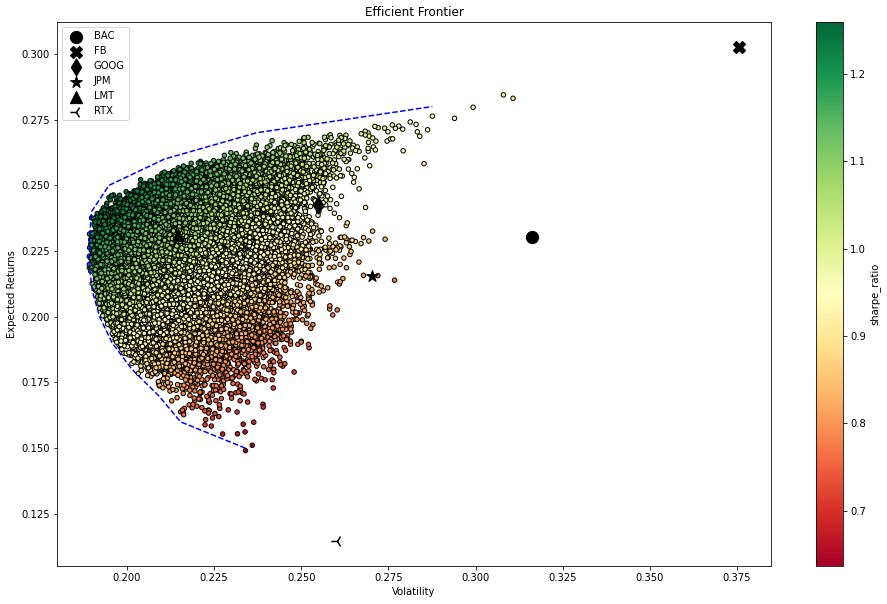
\includegraphics[width=1\textwidth]{portfolio_monte_carlo_1.png}
    \caption{Grafico con tutti i portafogli generati da Monte Carlo}
    \label{fig:pf_monte_carlo_1}
\end{figure}

\pagebreak

Dalle simulazioni eseguite identifichiamo vai portafogli che sono localizzati nella frontiera di efficienza, a figura \ref{fig:pf_monte_carlo_2} possiamo osservare
lo stesso grafico ma con evidenziati due portafogli sub-ottimali, uno con il rendimento più alto tra tutti e l'altro con la varianza più bassa.

\begin{figure}[ht]
    \centering
    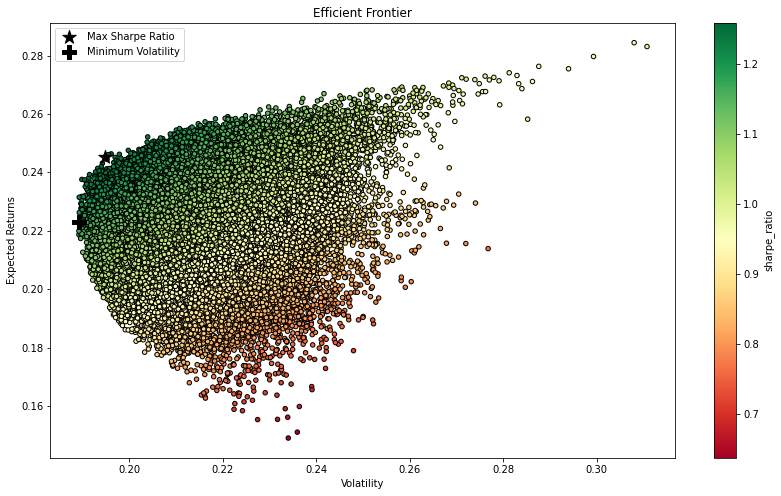
\includegraphics[width=1\textwidth]{portfolio_monte_carlo_2.png}
    \caption{Grafico con evidenza dei due portafogli sub-ottimali}
    \label{fig:pf_monte_carlo_2}
\end{figure}

La composizione del portafoglio sub-ottimale con il rendimento più alto la è la seguente (figura \ref{fig:pf_optimal_rd}).

\begin{figure}[ht]
    \centering
    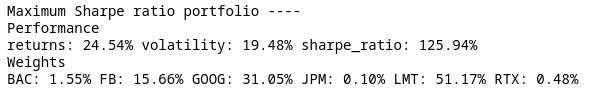
\includegraphics[width=.8\textwidth]{portfolio_optimal_rd.png}
    \caption{Composizione con pesi del portafoglio sub-ottimale con rendimento più alto}
    \label{fig:pf_optimal_rd}
\end{figure}

\textbf{Utilizzando i dati di previsione (portfolio di previsione)}

Applichiamo le simulazioni di Monte Carlo ai dati di previsione identificati nel capitolo 3 (su un periodo di 108 mesi).

La ripartizione della origine dei dati è la seguente:
\begin{itemize}
    \item Primi 80 mesi: Dati storici
    \item Dal mese 81 a 108: Dati di previsione
\end{itemize}

Dalle simulazioni usando oltre ai dati storici quelli di previsione otteniamo una dispersione dei portafogli notevolmente inferiore, a figura \ref{fig:prev_monte_carlo_1}
abbiamo i portafogli con la frontiera di efficienza evidenziata mentre a figura \ref{fig:prev_monte_carlo_2} vengono evidenziati come per il precedente grafico i due portafogli tale
per cui uno ha il rendimento più alto ed il secondo ha la volatilità più bassa.

\begin{figure}[p]
    \centering
    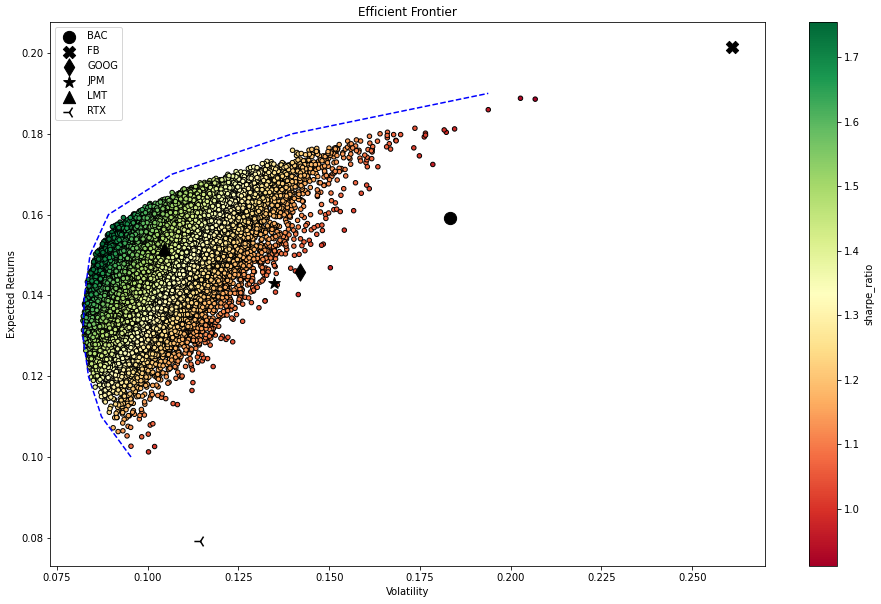
\includegraphics[width=1\textwidth]{portfolio_monte_carlo_prev_1.png}
    \caption{Grafico con tutti i portafogli generati da Monte Carlo usando dati di previsione}
    \label{fig:prev_monte_carlo_1}
\end{figure}

\begin{figure}[p]
    \centering
    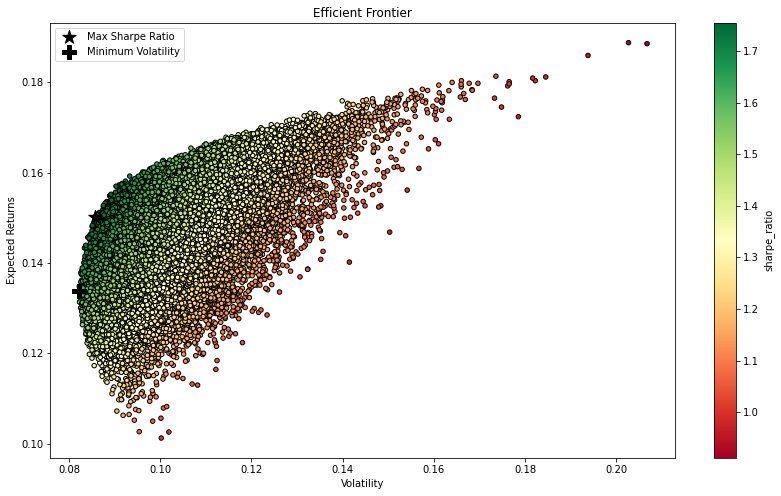
\includegraphics[width=1\textwidth]{portfolio_monte_carlo_prev_2.png}
    \caption{Composizione con pesi del portafoglio sub-ottimale con rendimento più alto usando i dati di previsione}
    \label{fig:prev_monte_carlo_2}
\end{figure}

\pagebreak

La composizione del portafoglio sub-ottimale con il rendimento più alto costituita al mese 80 con dati di previsione per
i successivi 27 mesi è la seguente (figura \ref{fig:pf_optimal_pr}).

\begin{figure}[ht]
    \centering
    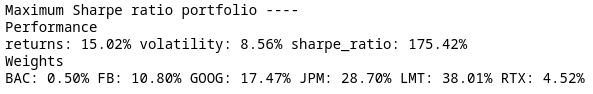
\includegraphics[width=.8\textwidth]{portfolio_optimal_pr.png}
    \caption{Composizione con pesi del portafoglio sub-ottimale con rendimento più alto usando i dati di previsione}
    \label{fig:pf_optimal_pr}
\end{figure}

Si può notare come l'utilizzo dei dati di regressione del modello \verb|ARIMA| abbia reso il valore di volatilità
notevolmente inferiore rispetto al portafoglio precedente a figura \ref{fig:pf_optimal_rd}.

\subsection{Beta dei portafogli ottimali}

L' indice beta per i due portafogli (dati passati e dati di previsione) è stato calcolato usando come per il punto 5 l'indice
\verb|S&P 500| (\verb|^GSPC|).

\subsubsection{beta del portfolio costituito solo con dati passati}

Sono stati considerati tutti i dati passati con cadenza giornaliera e mediante il metodo della regressione è stato calcolato il beta (figura \ref{fig:pf_optima_pd_beta_graph}).

\begin{figure}[ht]
    \centering
    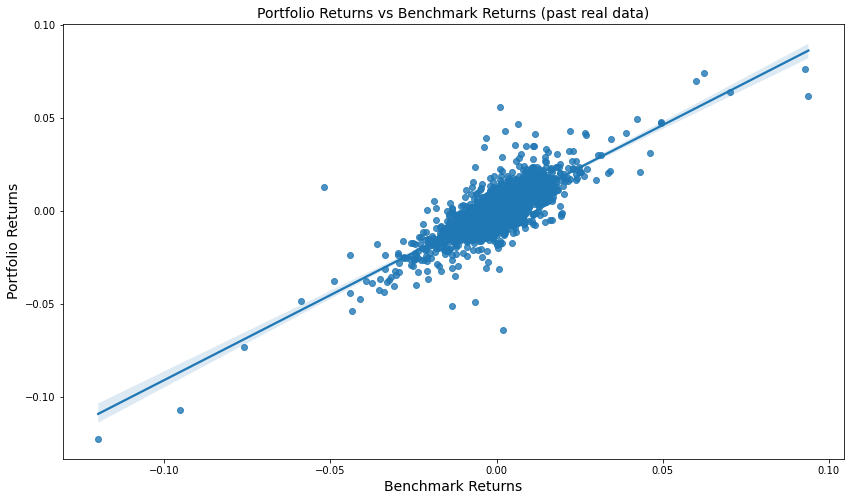
\includegraphics[width=.8\textwidth]{portfolio_beta_graph_pd.png}
    \caption{retta di regressione per calcolo del beta usando dati passati.}
    \label{fig:pf_optima_pd_beta_graph}
\end{figure}

L'indice beta calcolato è pari a \verb|0.9145|.

\pagebreak

\subsubsection{beta del portfolio costituito con dati di previsione}

In questo caso come per le sezioni precedenti per i 108 mesi sono stati usati sia i dati passati che quelli di previsione,
Rispetto al calcolo di beta effettuato qui sopra è stata considerata una frequenza mensile invece di giornaliera in quanto
il forecasting ha prodotto dati mensili (figura \ref{fig:pf_optima_pr_beta_graph}).

\begin{figure}[ht]
    \centering
    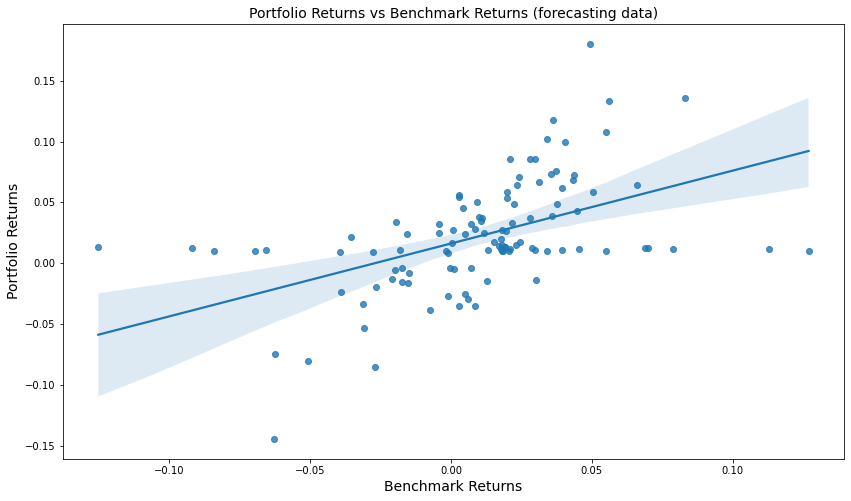
\includegraphics[width=.8\textwidth]{portfolio_beta_graph_pr.png}
    \caption{retta di regressione per calcolo del beta usando dati di previsione.}
    \label{fig:pf_optima_pr_beta_graph}
\end{figure}

L'indice beta calcolato è pari a \verb|0.5996|.

\subsection{Costruzione del portfolio effettivo e confronto}

Per la costruzione del portfolio effettivo si può usare la tecnica di allocazione chiamata \textbf{1/n portfolio}, questa
tecnica come da specifica del progetto alloca a tutti gli asset considerati peso uguale.\\
Nonostante il fatto che sembra una tecnica molto semplicistica è stato 
dimostrato  che può essere complicato superare la performance di un \verb|1\n portfolio| usando tecniche di asset allocation più complicate \cite{10.1093/rfs/hhm075}.

Per effettuare tutti i benchmark e ottenere la valutazione del portfolio è stata utilizzata la libreria \emph{pyfolio}.

\subsubsection{Dati reali passati}

Usando solo i dati reali passati si ottiene un tasso di rendimento annuale pari a $22.2\%$ con volatilità annuale del $20.09\%$, mentre con la costruzione
del portfolio usando Monte carlo abbiamo ottenuto un rendimento del $24.54\%$ ottenendo però una volatilità inferiore pari a $19.48\%$.

\subsubsection{Dati di previsione}

In questo caso come nelle sezioni precedenti sono stati usati dati passati e dati di previsione in congiunzione, considerando una limitazione di \emph{pyfolio} nei grafici di rendimento
cumulativo è presente un effetto "gradino" per la mancanza di informazioni tra i mesi.

Il tasso di rendimento annuale identificato è pari al $20.1\%$ mentre la volatilità $13.3\%$, con il metodo monte carlo si è identificato un portfolio con rendimento inferiore pari a $15.02\%$ ma con
volatilità inferiore pari a $8.56\%$.